% !TEX program = xelatex
\documentclass[hyperref,a4paper,UTF8]{ctexart}

\usepackage[left=2.50cm, right=2.50cm, top=2.50cm, bottom=2.50cm]{geometry}

\usepackage[unicode=true,colorlinks,urlcolor=blue,linkcolor=blue,bookmarksnumbered=true]{hyperref}
\usepackage{latexsym,amssymb,amsmath,amsbsy,amsopn,amstext,amsthm,amsxtra,color,bm,calc,ifpdf,booktabs}
\usepackage{graphicx}
\usepackage{enumerate}
\usepackage{fancyhdr}
\usepackage{listings}
\usepackage{multirow}
\usepackage{makeidx}
\usepackage{xcolor}
\usepackage{fontspec}
\usepackage{subfigure}
\usepackage{hyperref}
\usepackage{indentfirst}
\usepackage{amssymb}
\usepackage{float}
\usepackage{pythonhighlight}
\usepackage[ruled,linesnumbered]{algorithm2e}


\pagestyle{fancy}
\fancyhead[L]{}
\fancyhead[C]{\fangsong 云南大学信息学院机器学习实验(2023春)课程论文}
\fancyhead[R]{}

\renewcommand{\abstractname}{\textbf{\large {摘\quad 要}}} % 更改摘要二字的样式


\title{
机器学习实验(2023春)课程论文\\
~\\
\textbf{基于LightGCN的个性化动画推荐}
}
\author{
\kaishu\normalsize
姓名\ \underline{Steven} \qquad
学号\ \underline{} \qquad
}
\date{} % 留空,不显示日期

\begin{document}
\begin{figure}
    \centering
    
\includegraphics[width=0.7\textwidth]{fig/ynu.jpg}
\end{figure}
\maketitle



\begin{abstract}
    随着信息技术的发展,互联网已成为国民日常生活的重要组成部分。但互联网的海量信息在丰富人们生活的同时,也为人们筛选信息带来了困难。个性化推荐系统作为缓解大数据时代“信息过载”问题的有效工具,已成为目前构筑互联网生态的支撑技术之一。

    个性化推荐的核心之一是发掘用户意图。传统的启发式方法和基于矩阵分解的方法难以显式地捕捉更深层次的用户意图。由于推荐场景下的大部分数据本质上都是图结构的(如用户-物品的交互数据、用户的社交网络、物品的知识图谱等),图神经网络在个性化推荐算法方面展现出了较好的效果。

    本文从推荐系统出发,介绍了将交互数据以图结构建模,并介绍了如何将数据应用于LightGCN模型采用LightGCN模型,在mal数据集的约16万条交互数据下进行实验,完成模型的调试与训练;实现根据给定用户的特征推荐动画的功能。

    \noindent{\textbf{关键词:}LightGCN, 推荐系统, 图神经网络, 自监督学习}
\end{abstract}
\thispagestyle{empty} % 当前页不显示页码

\newpage % 目录页
\tableofcontents % 生成目录
\thispagestyle{empty} % 当前页不显示页码

\newpage % 索引页
\listoffigures % 生成插图索引

\listoftables % 生成表格索引

\thispagestyle{empty} % 当前页不显示页码

\newpage
\section{引言}
\subsection{研究内容}
本实验主要研究LightGCN应用于动画的个性化推荐方面的相关工作,工作内容大致包括:数据处理;搭建模型;训练、调整;调用预测四部分。
\subsection{结构安排}

本文结构安排如下:
\begin{enumerate}
    \item 第1章:引言,简单介绍进行的主要任务。
    \item 第2章:方法,主要介绍在实现该任务的过程中采用的方法及其原理。
    \item 第3章:实验,介绍该任务具体的实现流程,以及在实现方面的改进与技巧。
    \item 第4章:结果,介绍实验结束后的模型结果,以及演示实验模型进行预测。
    \item 第5章:总结,总结工作内容与收获。
\end{enumerate}


\section{方法}

\subsection{图与图嵌入}

\subsubsection{图}
现实中的很多数据很难以欧氏空间中的数学形式建模,如社交网络、分子结构等,这些数据通常是数据点的集合,且不同数据点之间存在某种关联。推荐系统所研究的两个主要对象:\textbf{用户}和\textbf{项目}正是这种数据,适合采用图结构为这两者的关系进行建模,以便于进行后续的研究。

图是一种数据结构,通常以$G=\{V,E\}$表示,其中$V$代表图中的节点集,每个点$v_i$表示其中的一个实体;$E$代表图中的边集,每个边$e_j$可以按照其是否有向分为有向边和无向边,边同时允许包含权重信息。

\begin{figure}[ht]
    \centering
    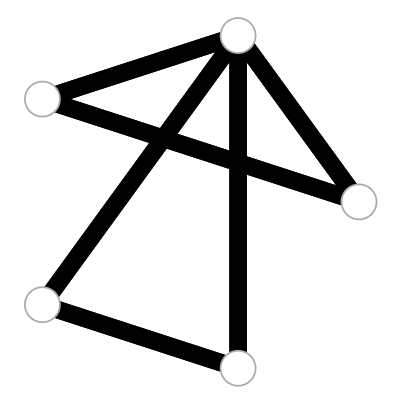
\includegraphics[width=0.3\textwidth]{fig/graph.jpg}
    \caption{图结构示意图}
    \label{fig:graph}
\end{figure}

在推荐系统中,$V$表示用户和项目,每个用户或项目都以一个点表示;$E$表示用户-项目之间的交互,边的权重定量的表示该交互的作用效果。在推荐系统中该类图也称为\textbf{用户-项目交互图}。

\subsubsection{图嵌入}
\textbf{嵌入}(Embedding)指将原始数据中多个距离空间中的数据嵌入到同一个距离空间,在实现形式上即从原始数据中提取特征,即数据映射\cite{embeddings}。在推荐系统中,通常将节点信息和交互信息都进行映射,并以向量表示。

\begin{figure}[ht]
    \centering
    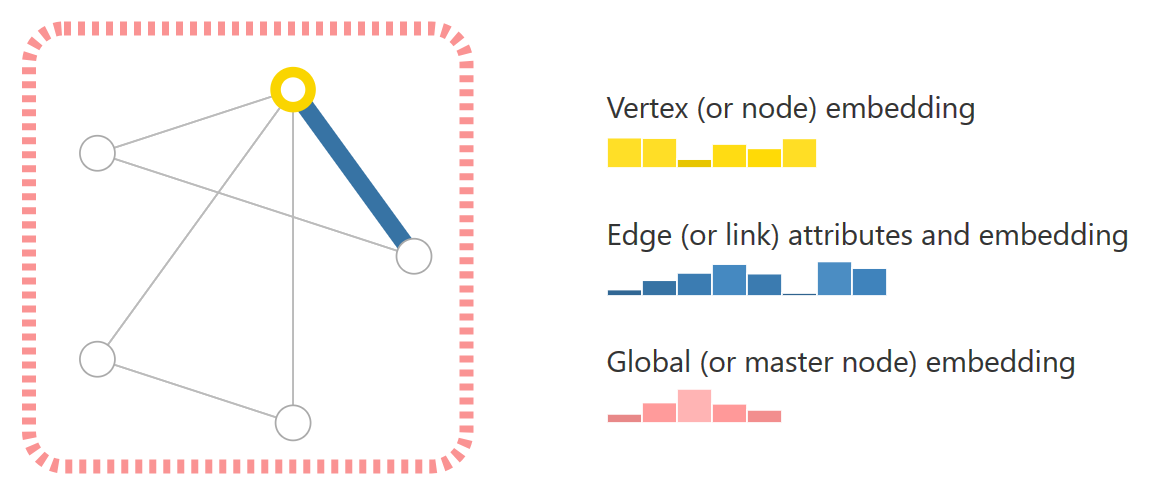
\includegraphics[width=0.7\textwidth]{fig/embedding.png}
    \caption{嵌入示意图}
    \label{fig:embedding}
\end{figure}


\subsection{卷积与GCN}

\subsubsection{卷积}
\textbf{卷积}是一种矩阵运算,运算过程为使用卷积核在数据上逐步滑动,并对卷积核覆盖的部分进行加权求和生成特征。该过程中权重即为卷积核,反映了对特征模式的偏好。卷积具有一些优秀的性质,如局部连接、参数共享、平移不变性等。

\subsubsection{GNN}
\textbf{GNN}即\textbf{图神经网络}。图神经网络的目标是通过学习节点的特征表示以推断节点之间的关系,以此进行节点分类、预测边的存在性等任务。

图神经网络的核心思想是通过\textbf{信息传递和聚合}对图中的节点进行表示学习。一般来说,图神经网络会为每个节点分配一个初始的Embedding,并通过消息传递和聚合过程来迭代更新节点。在每轮迭代中,节点会接收来自邻居节点的信息,并与自身的特征进行更新。

\subsubsection{GCN}
\textbf{GCN}即\textbf{图卷积网络},是一种用于处理图结构数据的图神经网络模型。

GCN借鉴了CNN的局部感知和权值共享的思想,通过邻居节点的信息传递和聚合来更新节点的表示。在GCN中,每个节点的表示是由该节点及其邻居节点的表示进行加权求和得到的,该过程大致可分为两步:

1. 聚合邻居节点的信息:将每个节点的特征向量与其邻居节点的特征向量进行加权求和,以得到聚合后的邻居节点信息。

2. 更新节点的表示:将聚合后的邻居节点信息与当前节点的特征向量进行融合,通过神经网络的非线性转换函数(如ReLU)进行更新,得到节点的新表示。

该过程的迭代公式可定义为\cite{kipf2017semisupervised}:

$$f(H^{(l)}, A) = \sigma(\hat{D}^{-\frac{1}{2}}\hat{A}\hat{D}^{-\frac{1}{2}} H^{(l)}W^{(l)}) $$

其中$\sigma$表示激活函数;$A$为邻接矩阵;$\hat{A}=A+I$,即在原始图中加入自环后的邻接矩阵,加入自环的目的是为了在Embedding更新时同时考量自身;$\hat{D}$表示$\hat{A}$的度矩阵;$H$表示各结点的Embedding,维度为$N\times embedding\_dim$,$W$为线性变化时所用的权重矩阵。

若对$A$进行规范化,则需要$A$的每一行除以对应行的和;但在邻接矩阵中,该值恰好等于该行所对应结点的度(degree),因此该过程中规范化可表示为:

$$A_{ij}=\frac{A_{ij}}{d_i},\text{or:}A=D^{-1}A$$

而在GCN模型中采用了对称规范化,公式表示为:

$$A_{ij}=\frac{A_{ij}}{\sqrt{d_i}\sqrt{d_j}},\text{or:}A=D^\frac{1}{2}AD^{\frac{1}{2}}$$

该过程对加入自环后的邻接矩阵$\hat{A}$进行规范化,并与$H^{(l)}$进行乘法,完成了消息聚合,再以$W^{(l)}$进行赋权;最后再通过激活函数得到$H^{(l+1)}$,完成结点表示(Embedding)的更新。

\begin{figure}[ht]
    \centering
    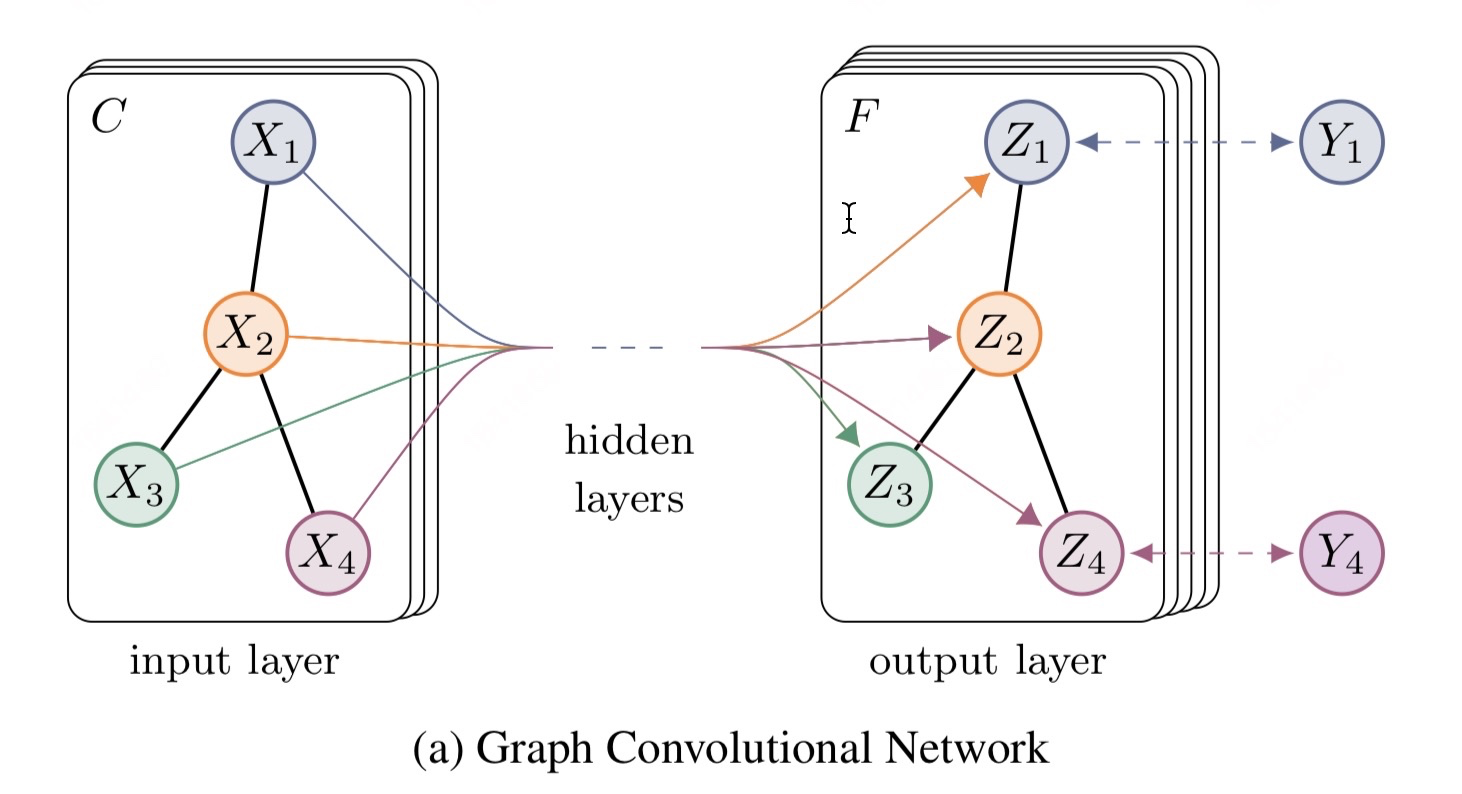
\includegraphics[width=0.6\textwidth]{fig/graph_conv.jpg}
    \caption{图卷积过程示意图}
    \label{fig:graph_conv}
\end{figure}

\subsection{LightGCN}
LightGCN是一种用于图神经网络的简化模型,相较于GCN,LightGCN去除了其中特征变化和非线性激活,而是直接使用简单的加权和聚合器来更新Embedding。

对于用户和项目,图卷积流程表示如下\cite{he2020lightgcn}:

$$e_u^{k+1}=\sum_{i\in N_u}\frac{1}{\sqrt{|N_u| |N_i|}}e_i^{(k)}$$

$$e_i^{k+1}=\sum_{u\in N_i}\frac{1}{\sqrt{|N_u| |N_i|}}e_u^{(k)}$$

其中$e_u$表示用户$u$的Embedding,$e_i$表示项目$i$的Embedding;$N_i$表示与用户$u$交互的邻居项目$i$,$N_u$表示与项目$i$交互的邻居用户$u$。从公式不难看出,这实际相当于一种平滑过程:迭代地根据邻居结点的Embedding平滑自身的Embedding。

LightGCN是一个迭代算法,若迭代次数记为$K$,在迭代完成后,一个用户/项目的最终嵌入表示为:

$$e_u=\sum^K_{k=1}\alpha_k e_u^{(k)}$$
$$e_i=\sum^K_{k=1}\alpha_k e_i^{(k)}$$

其中$\alpha_k$表示第$k$层Embedding的权重,根据\cite{he2020lightgcn}的研究结果表示,$\alpha_k$统一设为$\frac{1}{K+1}$时效果较好,因此在模型中并未设置策略动态调整$\alpha_k$的值。若以矩阵表示则为$E=\alpha_0E^{(0)}+\alpha_1E^{(1)}+\cdots +\alpha_K E^{(K)}=\alpha_0 E^{(0)}+\alpha_1\hat{A}E^{(0)}+\cdots +\alpha_K \hat{A}^{(K)} E^{(0)}$


此外,LightGCN属于“自监督学习”,因为LightGCN处理的数据并没有或只有很少的标记。LightGCN引入了基于最大化相似性的目标函数,通过最大化正样本之间的相似性和最小化负样本之间的相似性来学习节点嵌入表示。这种自监督学习的思想使得 LightGCN 能够从图结构中自动学习节点的表示,而无需额外的标签信息。
\subsection{BPR Loss}
假定用户的历史行为可以表示为一个三元组$(u,i,r)$,其中$u$表示用户,$i$表示物品,$r$表示用户对物品的反馈。

BPR模型的目标是学习到一个针对每个用户$u$的排序函数$f_u(i)$,该函数能够将物品按照用户的偏好降序排序;而损失函数的思想为:若对于一个用户$u$和两个物品$i,j$,BPR损失函数应当让用户更喜欢的物品$i$排在用户更不喜欢的物品$j$之前,这等价于最大化如下边界概率\cite{rendle2012bpr}:

$$P(u_{i>j}) = \sigma(f_u(i) - f_u(j))$$

其中,$u_{i>j}$ 表示在用户 $u$ 的偏好下,物品 $i$的排名高于物品 $j$,$\sigma$ 是 $sigmoid$ 函数。为了最大化上述的边际概率,BPR损失函数可以被定义为\cite{rendle2012bpr}:

$$L_{BPR} = -\sum_{(u, i, j) \in D} \ln \sigma(f_u(i) - f_u(j))$$

其中,$D$ 表示训练集中的所有三元组,$f_u(i)$ 表示用户 $u$ 对物品 $i$ 的偏好得分。这个公式很好理解,我们希望对于 $i$ 的得分尽可能大于 $j$ 的得分,也就是希望 $f_u(i)-f_u(j)$ 的差大于$0$且尽可能大,又由于 $\sigma$ 激活函数的特点是横坐标越大,$y$值越接近$1$,那么偏好分的差越大,经过 $\sigma$ 之后的结果越靠近$1$,再送入 $\ln$ 函数中也就会越接近$0$,反之越大,因为 $\sigma$ 的值域为$0-1$,所以经过$\ln$之后的值为负数,为了表示损失所以在前面添加负号。

\section{实验}
\subsection{环境配置}
\begin{itemize}
    \item \textbf{OS}: EndeavourOS \textbf{6.3.9-arch 1-1}(Based on ArchLinux)
    \item \textbf{数据集}:\hyperlink{https://www.kaggle.com/datasets/shafiwalsher/myanimelist-dataset-2023-top-15000}{mal-anime}
    \item \textbf{Python} 3.11.3
    \item \textbf{torch} 2.0.1+cu118
    \item \textbf{torch\_geometric} 2.3.1
\end{itemize}

此外,由于\pyth{torch_geometric.utils.structured_negative_sampling()}函数存在部分缺陷,因此在本地运行时修改了该函数部分内容,修改后的该函数定义如下:

\begin{python}
    def structured_negative_sampling(edge_index, num_nodes: Optional[int] = None, contains_neg_self_loops: bool = True):
        num_nodes = maybe_num_nodes(edge_index, num_nodes)
    
        row, col = edge_index.cpu()
        pos_idx = row * num_nodes + col
        if not contains_neg_self_loops:
        loop_idx = torch.arange(num_nodes) * (num_nodes + 1)
        pos_idx = torch.cat([pos_idx, loop_idx], dim=0)
    
        rand = torch.randint(edge_index[1].min(),edge_index[1].max(), (row.size(0), ), dtype=torch.long)
        neg_idx = row * num_nodes + rand
    
        mask = torch.from_numpy(np.isin(neg_idx, pos_idx)).to(torch.bool)
        rest = mask.nonzero(as_tuple=False).view(-1)
        while rest.numel() > 0:  # pragma: no cover
        tmp = torch.randint(edge_index[1].min(),edge_index[1].max(), (rest.size(0), ), dtype=torch.long)
        rand[rest] = tmp
        neg_idx = row[rest] * num_nodes + tmp
    
        mask = torch.from_numpy(np.isin(neg_idx, pos_idx)).to(torch.bool)
        rest = rest[mask]
    
        return edge_index[0], edge_index[1], rand.to(edge_index.device)

\end{python}

\subsection{数据处理}
本节主要介绍实验中关于数据处理部分的大致工作。

1. 首先使用\pyth{pandas.read_csv()}函数读取两个csv文件:anime.csv和rating\_anime.csv,并进行数据预处理,去除无rating的anime,去除无对应anime的rating,将处理后的数据定义为\pyth{user_mapping, anime_mapping, edge}三个变量。

2. 随后使用\pyth{sklearn.model_selection.train_test_split()}函数划分训练集、测试集、验证集

3. 最后使用\pyth{torch_sparse.SparseTensor},将这三类数据转换为稀疏矩阵类型,以便于运算。

\begin{figure}[ht]
    \centering
    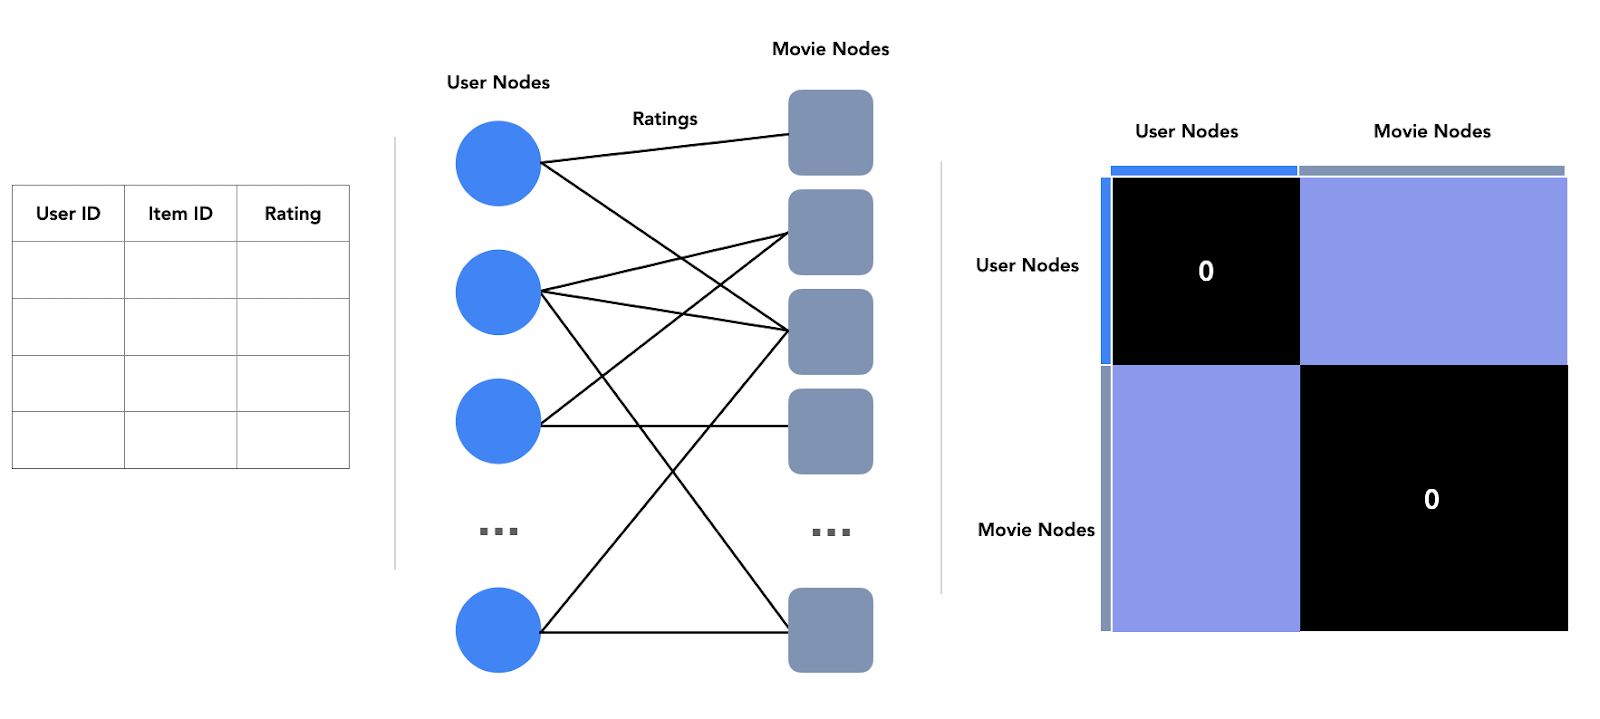
\includegraphics[width=0.8\textwidth]{fig/sparse_matrix.png}
    \caption{以稀疏矩阵表示图结构}
    \label{fig:sparse_matrix}
\end{figure}

\subsection{模型定义}
本节主要介绍实验中关于模型搭建的大致工作。

1. 首先继承\pyth{torch_geometric.nn.conv}中的\pyth{MessagePassing}类,并在此基础上实现了对user和item从原始数据向embedding向量的转化。

2. 在\pyth{forward()}方法中实现了上述Embedding矩阵的更新过程,从$E^{(k)}$计算出$E^{(k+1)}$
\subsection{运行结果}

本次实验共迭代8000次,每200次计算一次loss、precision、recall和ncdg值,结果如下:

\begin{figure}[ht]
    \centering
    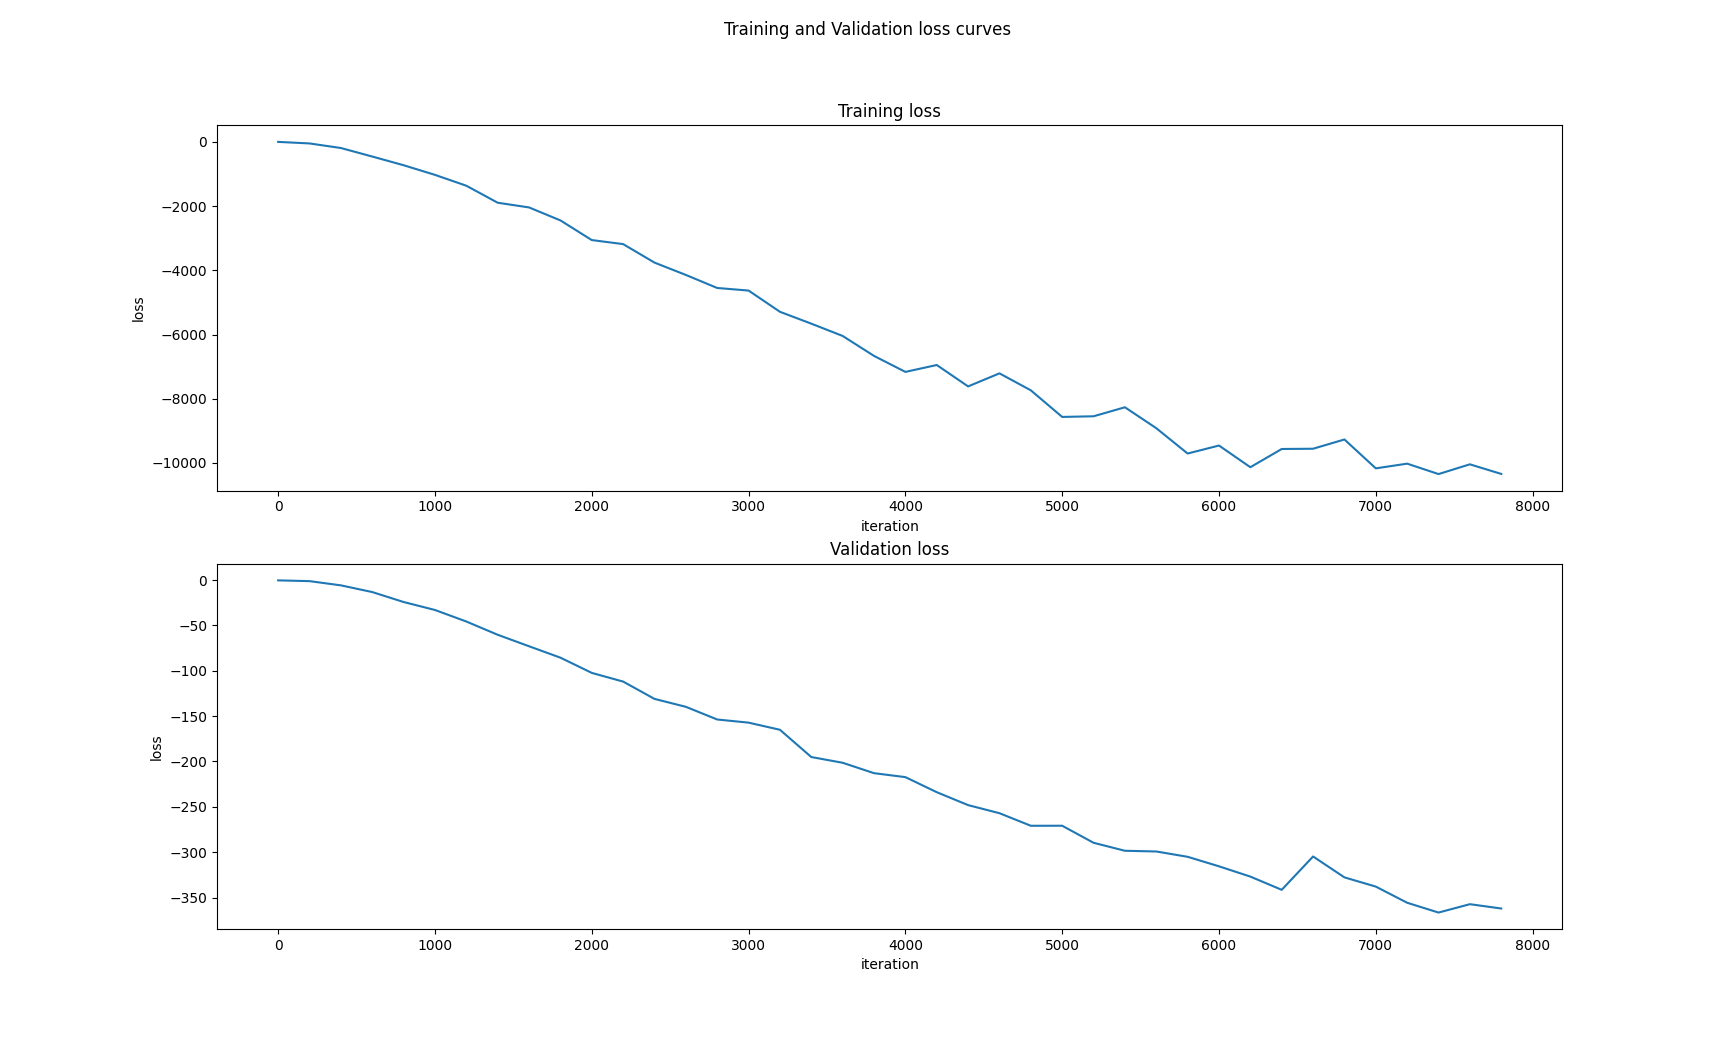
\includegraphics[width=1.0\textwidth]{fig/loss.png}
    \caption{损失函数变化}
    \label{fig:loss}
\end{figure}

\section{结果}
\subsection{模型训练}

迭代过程中输出信息如表\ref{tab:model_trsain_result}所示

\begin{table}[ht]
    \centering
    \begin{tabular}{l|c|c|c|c|c|}
        \toprule
        iteration & train\_loss  & val\_loss   & val\_ncdg \\
        \hline  %在第一行和第二行之间绘制横线
        200       & -0.69127     & -0.40227    & 0.00141   \\
        400       & -48.91718    & -1.24899    & 0.00211   \\
        600       & -191.42261   & -5.89279    & 0.00225   \\
        800       & -456.82629   & -13.27942   & 0.00223   \\
        1000      & -727.495     & -24.25015   & 0.00222   \\
        1200      & -1027.33374  & -33.03998   & 0.00225   \\
        1400      & -1365.72729  & -45.74011   & 0.00231   \\
        1600      & -1895.22986  & -60.34967   & 0.00229   \\
        1800      & -2041.81665  & -73.01404   & 0.00246   \\
        2000      & -2445.69067  & -85.57806   & 0.00245   \\
        2200      & -3058.07739  & -102.36475  & 0.00238   \\
        2400      & -3183.82666  & -111.93848  & 0.00244   \\
        2600      & -3759.76636  & -131.01379  & 0.00249   \\
        2800      & -4144.05371  & -139.75391  & 0.00256   \\
        3000      & -4550.22021  & -153.72473  & 0.00254   \\
        3200      & -4630.38818  & -157.19543  & 0.00254   \\
        3400      & -5291.74951  & -165.0542   & 0.00256   \\
        3600      & -5661.37061  & -195.09082  & 0.00255   \\
        3800      & -6043.92383  & -201.41113  & 0.00252   \\
        4000      & -6665.50635  & -212.87329  & 0.00258   \\
        4200      & -7163.50635  & -217.2373   & 0.00261   \\
        4400      & -6948.5459   & -233.83301  & 0.00264   \\
        4600      & -7615.39355  & -248.07861  & 0.0026    \\
        4800      & -7209.08301  & -256.99487  & 0.00258   \\
        5000      & -7737.37402  & -270.84204  & 0.00259   \\
        5200      & -8565.79883  & -270.80664  & 0.00262   \\
        5400      & -8545.57227  & -289.59033  & 0.0026    \\
        5600      & -8264.9541   & -298.39551  & 0.00259   \\
        5800      & -8916.33887  & -299.17749  & 0.00257   \\
        6000      & -9705.64355  & -305.0376   & 0.00256   \\
        6200      & -9456.79004  & -315.5249   & 0.0026    \\
        6400      & -10131.67871 & -326.86523  & 0.00259   \\
        6600      & -9564.26953  & -341.42603  & 0.00259   \\
        6800      & -9556.08594  & -304.67896  & 0.00258   \\
        7000      & -9267.91895  & -327.71118  & 0.00258   \\
        7200      & -10167.37598 & -337.87354  & 0.00259   \\
        7400      & -10020.85352 & -355.68335  & 0.00258   \\
        7600      & -10345.22559 & -366.47656  & 0.0026    \\
        7800      & -10041.59863 & -357.26538  & 0.0026    \\
        8000      & -10340.8291  & -362.01709  & 0.0026    \\
        \bottomrule
    \end{tabular}
    \caption{模型训练结果}
    \label{tab:model_trsain_result}
\end{table}

\subsection{预测结果}

在执行完毕后,调用保存的模型,并进行推理,结果如下:

\begin{figure}[ht]
    \centering
    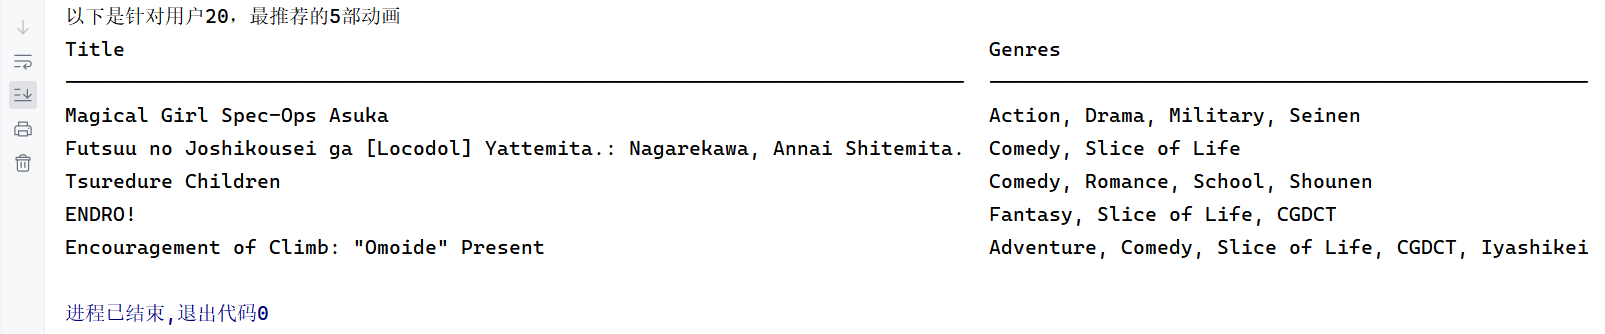
\includegraphics[width=1.0\textwidth]{fig/predict.png}
    \caption{预测结果}
    \label{fig:predict}
\end{figure}


\section{总结}

本次实验完成了基于LightGCN的个性化动画推荐系统,实现根据给定用户的特征推荐动画的功能。

通过本次实验,我学习了推荐系统与图神经网络的相关思想及公式推导,深入理解了LightGCN的模型改进和设计理念,同时也了解了当前图结构数据在计算机上如何处理以及困难,对神经网络又有了更多的观察和思考的角度。


\newpage
\bibliographystyle{acm}
\bibliography{reference}

\end{document}
